\begin{surferIntroPage}{Simple Singularities}{simplesing_A1pm}{Simple Singularities}
	Surfaces like the sphere and the torus shown below are called non-singular or smooth. They all look like a plane in a small neighborhood of each point and do not contain any apex, self-intersection or pieces meeting tangentially. In contrast, the examples on the right have non-smooth points. They are called singular or singularities.
	\begin{center}%
		smooth:\enspace%
		\raisebox{-0.5\height}{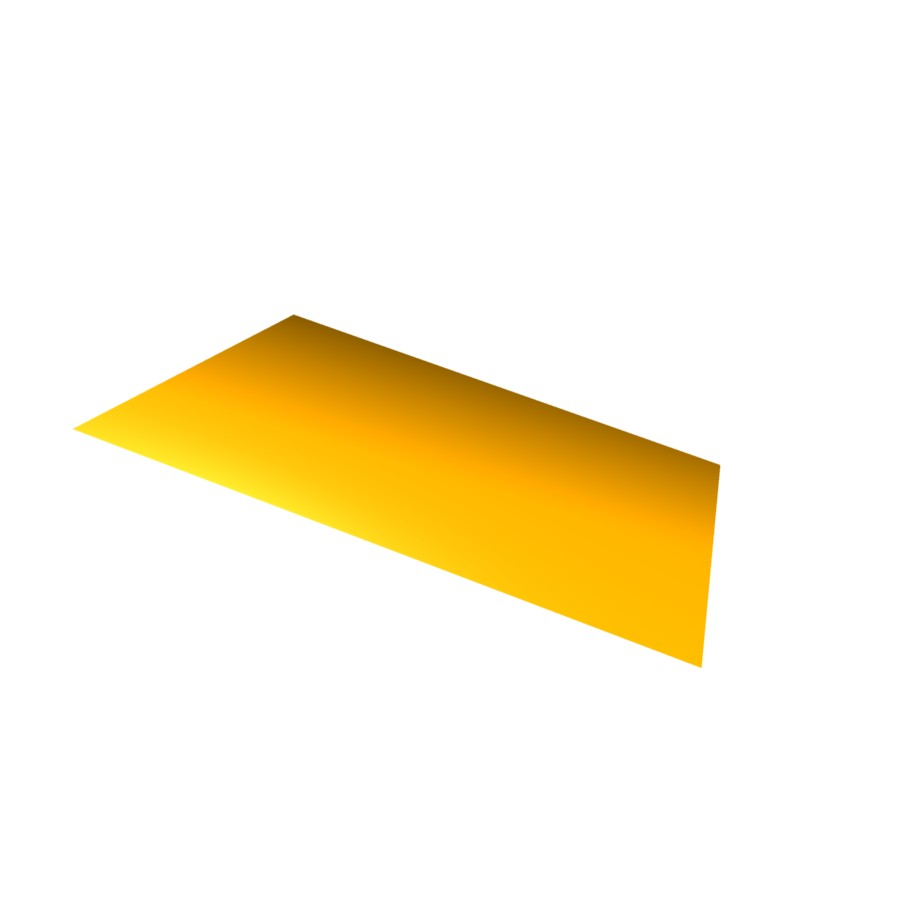
\includegraphics[width=1.1cm]{../../common/images/plane}}%
		\raisebox{-0.5\height}{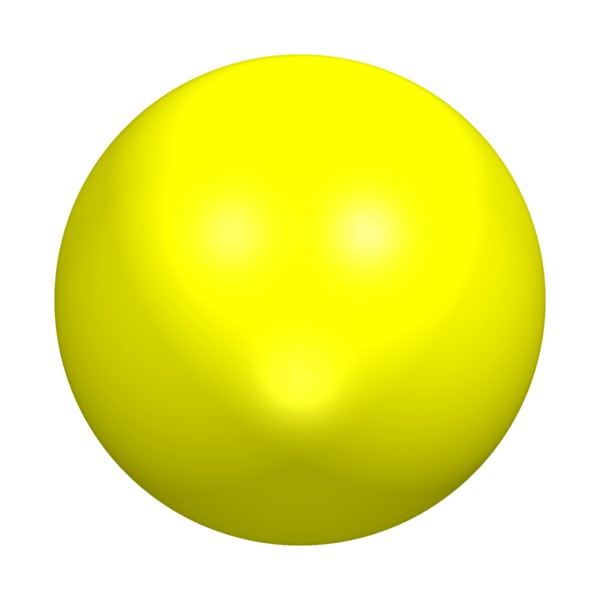
\includegraphics[width=1.1cm]{../../common/images/kugel}}%
		\raisebox{-0.5\height}{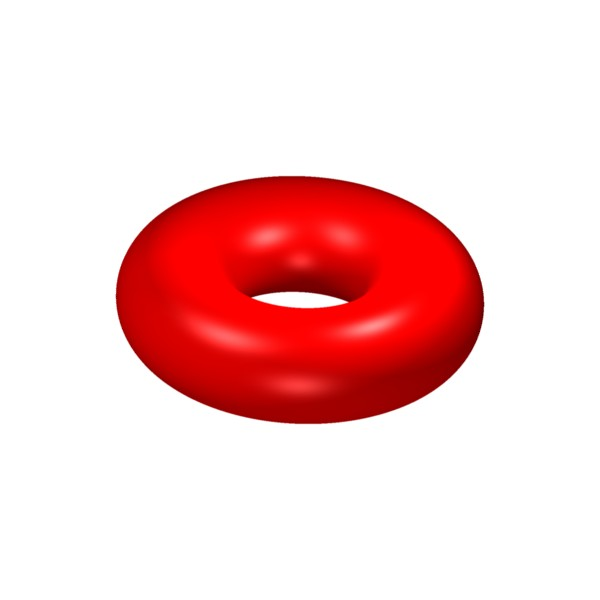
\includegraphics[width=1.1cm]{../../common/images/torus}}%
        \quad%
		singular:%
		\raisebox{-0.5\height}{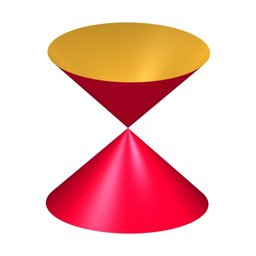
\includegraphics[width=1.1cm]{../../common/images/kegel}}%
		\raisebox{-0.5\height}{\includegraphics[width=1.1cm]{../../common/images/A2pm}}%
		\raisebox{-0.5\height}{\includegraphics[width=1.1cm]{../../common/images/A3pm_0}}%
	\end{center}
	This gallery visualizes the most important class of singularities of algebraic surfaces, the so-called Simple or ADE-Singularities, which have amazing relations to numerous different areas of mathematics, to mathematical physics and to real life (e.g. in geometric optics). They are given by the infinite series $A_k^{\pm\pm}\!$, $k\geq 1$, $D_k^{\pm\pm}\!$, $k\geq 4$, and the three singularities $E^\pm_6\!, E^\pm_7\!, E^\pm_8\!$.

	Using SURFER, everyone can visualize these singularities. However, pictures of different singularities can look very similar, hiding their actual complexity. It is much better to deform the equation slightly in a special way and to visualize the deformed surface. For example, each $A_k$ singularity can be deformed into $\lfloor\frac{k+1}{2}\rfloor$ $A_1$ singularities. For an $A_3^{+-}$, we obtain two $A_1^{+-}$ as shown in the three pictures on the left:
	\vspace{-0.2cm}
	\begin{center}%
		\includegraphics[width=1.2cm]{../../common/images/A3pm_0}\enspace%
		\includegraphics[width=1.2cm]{../../common/images/A3pm_1}\enspace%
		\includegraphics[width=1.2cm]{../../common/images/A3pm_2}\enspace%
		\qquad\quad%
		\raisebox{1mm}{\includegraphics[width=1.2cm]{../../common/images/A3pm_vz_2}}\enspace%
		\raisebox{1mm}{\includegraphics[width=1.2cm]{../../common/images/A3pm_vz_1}}\enspace%
		\includegraphics[width=1.2cm]{../../common/images/A3pm_vz_0}
	\end{center}
	\vspace{-0.2cm}
	The index $k$ of an $A_k$ singularity is its so-called \emph{Milnor Number}. It is the number of \emph{holes} which vanish when contracting them to the singular point. This kind of deformation is shown on the right.
\end{surferIntroPage}
